\documentclass[11pt, oneside]{article}   	% use "amsart" instead of "article" for AMSLaTeX format
\usepackage{geometry}                		% See geometry.pdf to learn the layout options. There are lots.
\geometry{letterpaper}                   		% ... or a4paper or a5paper or ... 
%\geometry{landscape}                		% Activate for rotated page geometry
%\usepackage[parfill]{parskip}    		% Activate to begin paragraphs with an empty line rather than an indent
\usepackage{graphicx}				% Use pdf, png, jpg, or eps§ with pdflatex; use eps in DVI mode
								% TeX will automatically convert eps --> pdf in pdflatex	
\graphicspath{ {white-paper-figures/} }	
\usepackage{amssymb}
\usepackage{amsmath}
\usepackage{siunitx}
\sisetup{group-separator = {,}}

%SetFonts

%SetFonts


\title{Optimal Inventory Allocation for E-commerce Fulfillment}
\author{Christopher Holloman \\ Chief Data Scientist \\ Advanced Analytics Practice \\ Information Control Company}
\date{Last updated: \today}							% Activate to display a given date or no date

\begin{document}
\maketitle

Over the past several years, the importance of e-commerce to traditional retailers has grown dramatically.  While shoppers still purchase goods from brick-and-mortar stores regularly, Amazon and other on-line retailers have taken a significant amount of business from traditional stores.  All retailers must serve customers online to survive, and it's important that they are able to meet the same standards for delivery speed as online-only retailers.

One of the key aspects of meeting these high standards is to optimally allocate inventory to fulfillment centers to ensure that goods can be delivered to customers' home addresses quickly.  Optimal allocation must account for two primary factors:

\begin{itemize}
\item Cost of delivering units from fulfillment centers to delivery addresses
\item Cost of transferring units between fulfillment centers to respond to shifts in demand
\end{itemize}

We present a strategy for allocating units for a single SKU to an arbitrary number of fulfillment centers.

\section{Assumptions}

There is a long process from determining which styles a retailer will sell to determining exactly how those styles are delivered to customers.  Among the problems to be solved along the way are the following:

\begin{itemize}
\item How to forecast the number of units to be sold
\item How to forecast the fraction of units sold in different regions
\item How to quantify the uncertainty about the number of units to be sold
\item How to determine the number of units to allocate to each store
\item How to determine the number of units to store in each distribution center
\item How to determine the number of units to place in each e-commerce fulfillment center
\item How to determine which e-commerce fulfillment center fills each order
\item How to determine when units are shipped from one e-commerce fulfillment center or distribution center to another
\end{itemize}

For the purpose of this paper, we assume that the retailer has already developed a statistical model forecasting the number of units that will be purchased through the online channel in each of several regions.  We also assume the retailer has quantified their uncertainty in those forecasts.  Further, we assume that the retailer has a set of rules specifying the logic for fulfilling orders from fulfillment centers and for transferring units between fulfillment centers.

\section{Forecasting Online Sales}

When forecasting on-line sales, we start with a set of households, denoted $\mathcal{H}$.  When performing forecasting, we usually create forecasts not for individual households but for groups of households.  For example, we might create forecasts within political boundaries (\emph{e.g.,} county or state) or within designated marketing areas.  Define a partition $\mathcal{P}$ of $\mathcal{H}$, so $\mathcal{P} = \{P_1, P_2, ..., P_K \}$, where $P_k \cap P_{k'} = \emptyset$ for all $k$ and $k'$ and $\bigcup_k P_k = \mathcal{H}$.  The elements of this partition constitute the set of regions for which forecasts are created.

For simplicity of modeling, we assume that forecasting for the SKU of interest has been performed taking a Bayesian approach, so the retailer has posterior distributions for each of the parameters in the forecasting model.  Denote the historical demand data from which the forecasting model was constructed $\mathbf{Y}$ and the historical independent variables used to predict demand $\mathbf{X}$.  Denote the set of parameters in the model $\boldsymbol{\theta}$.  Using a Bayesian approach, the forecasting model has a posterior distribution for $\boldsymbol{\theta}$,

$$\pi (\boldsymbol{\theta} \mid \mathbf{Y}, \mathbf{X}) \propto \pi (\mathbf{Y} \mid \boldsymbol{\theta}, \mathbf{X}) \pi (\boldsymbol{\theta}).$$

\noindent For the purpose of forecasting future sales, we assume that future values of the independent variables are known.  We denote those future values $\mathbf{X}^*$.  Similarly, we denote future values of demand $\mathbf{Y}^*$.  The predictive distribution of $\mathbf{Y}^*$ is

$$\pi (\mathbf{Y}^* \mid \mathbf{X}^*, \mathbf{Y}, \mathbf{X}) = \int_{\boldsymbol{\Theta}} \pi (\mathbf{Y}^* \mid \boldsymbol{\theta}, \mathbf{X}^*) \pi (\boldsymbol{\theta} \mid \mathbf{Y}, \mathbf{X}) d \boldsymbol{\theta}$$.

\noindent We assume that forecasting is performed over a finite set of time points, $1, \ldots, T$ within each region.  The forecast in region $k$ at time $t$ is denoted $Y_{kt}^*$.  The total demand across all time points and regions is denoted $D^*$, and

$$D^* = \sum_{t = 1}^T \sum_{k = 1}^K Y_{kt}^*$$

\section{Determining the Buy}

For our determination of optimal allocation, we assume that the number of units purchased has already been determined.  Denote the total number of units purchased $b$.  Typically, the actual buy is selected to ensure a low probability that demand exceeds supply.  For example, we might select the $95^{th}$ percentile of the predictive distribution of $D^*$, giving a $5\%$ probability that demand will exceed supply.

\section{Fulfillment Centers}

Denote the set of fulfillment centers for e-commerce orders $\mathcal{F}$.  We use $J$ to denote the total number of fulfillment centers in $\mathcal{F}$.

\section{Cost functions}

There are two primary factors associated with optimal allocation

\begin{itemize}
\item Cost of delivering units from fulfillment centers to delivery addresses
\item Cost of transferring units between fulfillment centers to respond to shifts in demand
\end{itemize}

Each of these is a function.  The first is a function of household location and fulfillment center location, with distances between the two generally being associated with greater cost for delivery.  Denote this cost function $c_1 \colon \mathcal{F} \times \mathcal{H} \mapsto \mathbb{R}^+$.  The second is a function of the two fulfillment center locations.  As with $c_1$ the cost typically increases with distance, but in this case it may also increase with the number of units shipped between the two locations.  Denote this cost function $c_2 \colon \mathcal{F}^2 \times \mathbb{I}^+ \mapsto \mathbb{R}^+$.

These functions may be complicated, but they are typically straightforward linear equations with fixed and variable cost components.  Denote the distance (in miles, time, or other unit convenient for describing shipping cost) between two points $d(\cdot, \cdot)$.  Then, a typical function for delivery would be

$$c_1 (f, h) = \gamma_{11} + \gamma_{12} d(f, h),$$

\noindent where $\gamma_{11}$ and $\gamma_{12}$ are positive values representing fixed cost and variable cost associated with distance travelled, respectively.  A typical function for transfer would be

$$c_2 (u, f_1, f_2) = \gamma_{21} + \gamma_{22} u + \gamma_{23} d(f_1, f_2),$$

\noindent where $u$ is the number of units shipped, and $\gamma_{21}$, $\gamma_{22}$, and $\gamma_{23}$ are positive values representing fixed cost and variable cost associated with number of units shipped and distance travelled, respectively.

\section{Fulfillment and Transfer Rules}

Each business is unique in determining the rules it follows for fulfillment and transfer.  Fulfillment rules specify how each household placing an order will be assigned to the fulfillment center that will fulfill the order.  Transfer rules specify when transfers of units will be made between fulfillment centers.  We assume that these rules have been specified by the business and are not being optimized as part of the allocation optimization problem.

\section{Markdowns}

Retailers use markdowns to dispose of inventory that remains after the total demand for the full-price product has been exhausted.  When $d^* < b$, there are $b - d^*$ excess units to be marked down by the business.  These units are typically sold a price resulting in a lower AUR than for the full-price product.  We assume that the AUR for excess units can be expressed using a function $m \colon \mathbb{I}^2 \mapsto \mathbb{R}^+$.  A typical function for markdown would be

$$m (b, d^*) = r \exp \{- \delta (b - d^*) \},$$

\noindent where $r$ is the AUR for full-price units before demand is exhausted and $\delta$ is a parameter controlling how much markdown is required to dispose of excess inventory.

\section{Initial Allocation and Value}

For each of the $J$ fulfillment centers, our goal is to specify the number of units to be initially placed in each fulfillment center.  Let $\alpha_{jt}$ denote the inventory in fulfillment center $j$ at time $t$.  The initial allocation to fulfillment center $j$ is denoted $\alpha_{j0}$.

Given an initial allocation, a set of fulfillment and transfer rules, a set of cost functions, an AUR value, a formula for markdown AUR, and a set of known demand values, it is possible to calculate a total value for an allocation rule as

\begin{align*}
\nu(\alpha_{10}, \alpha_{20}, \ldots, \alpha_{J0}, \mathbf{y}^*) = &br \mathrm{I}_{\{b \leq d^*\}} \\
&+ \left( d^*r + m(b, d^*) \} \right) \mathrm{I}_{ \{ b > d^* \} } \\
&+ \sum_{t = 1}^T \sum_{k = 1}^K \sum_{i = 1}^{n_{kt}} c_1 (f_{tki}, h_{tki}) \\
&+ \sum_{a = 1}^A c_2 (f_{a1}, f_{a2}, u_a),
\end{align*}

\noindent where $\mathrm{I}_{\{ \cdot \}}$ is the indicator function taking a value of $1$ if its subscript is true and $0$ otherwise, $n_{kt}$ is the number of households in region $k$ placing orders at time $t$, $h_{tki}$ is the $i^{th}$ household placing an order in region $k$ at time $t$, $f_{tki}$ is the fulfillment center delivering to household $h_{tki}$, and $A$ is the total number of transfers made between fulfillment centers.  The first line of the equation is the total sales value (number of units bought time AUR) when fewer units are purchased than the amount of demand at full price.  The second line is the total sales value when more units are purchased than the number for which there is demand at full price.  The third line is the cost of delivery.  The fourth line is the cost of transfers.

While it is possible to calculate the value if future purchases are known, the future purchases are a random variable.  Consequently, instead of optimizing value, we optimize expected value, $\mathbb{E}[\nu]$.

$$\mathbb{E}[\nu \mid \alpha_{10}, \alpha_{20}, \ldots, \alpha_{J0}] = \int_{\mathbf{Y}^*} \nu(\alpha_{10}, \alpha_{20}, \ldots, \alpha_{J0}, \mathbf{Y}^*) \pi (\mathbf{Y}^* \mid \mathbf{X}^*, \mathbf{Y}, \mathbf{X}) d \mathbf{Y}^*$$.

\section{Implementation}

Calculation of $\mathbb{E}[\nu]$ for an initial allocation is intractable for even the simplest fulfillment and transfer rules.  Instead, we perform the optimization using a Monte Carlo approach.  The approach can be summarized as follows:

\begin{enumerate}
\item Generate a list of potential initial allocation values $\boldsymbol{\alpha}^{(1)}, \boldsymbol{\alpha}^{(2)}, \ldots, \boldsymbol{\alpha}^{(G)}$.
\item Loop through the sets of allocation values $g = 1, 2, \ldots, G$.
\begin{enumerate}
\item Loop through multiple iterations $l = 1, 2, \ldots, L$.
\begin{enumerate}
\item Generate a random draw of $\boldsymbol{\theta}$ from its posterior distribution.
\item Generate a random draw of $\mathbf{Y}^*$ from its posterior distribution, conditional on the drawn value of $\boldsymbol{\theta}$.
\item Loop through time points executing the fulfillment and transfer rules.
\item Record total value obtained.
\end{enumerate}
\item Average the $L$ calculated total values to obtain an estimate of expected total value.
\end{enumerate}
\item Select the initial allocation combination with the greatest expected total value.
\end{enumerate}

\section{Example}

\subsection{Problem Setup}

As a proof of concept, we implemented the recommended strategy on a simulated dataset.  A set of \SI{10000} households were generated and randomly assigned a location on the unit square.  Four fulfillment centers were also randomly assigned locations on the unit square.  The households were grouped into eight regions.  The locations of households, their assigned regions, and the locations of the fulfillment centers are shown in Figure~\ref{fi:hhfclocs}.

\begin{figure}
\centering
\includegraphics{hh-fc-locations}
\caption{Household locations (colored dots) by region with fulfillment center locations (numbers).}  \label{fi:hhfclocs}
\end{figure}

Within each of the eight regions, we specified a data distribution consisting of a Poisson distribution with a mean following an exponential decay curve.

$$Y_{kt}^* \mid \boldsymbol{\theta}_{k} \sim Poi(\mu_{kt})$$
$$\mu_{kt} = \theta_{1k} \exp \{ -t / \theta_{2k} \}.$$

\noindent We note that this model is somewhat simplistic since observations are conditionally independent, a scenario which is unlikely in a real forecasting situation.

Rather than generate values of $\mathbf{Y}$ and derive posterior distributions for the $\boldsymbol{\theta}$ parameters, we directly specified a hypothetical posterior distribution for each parameter.  The $95\%$ credible intervals for the cumulative demand curve derived from those posterior distributions in each region is shown in Figure~\ref{fi:demcurve}.  For this example, we set $T = 100$, so the demand curve is shown for $t = 1, 2, \ldots, 100$.

\begin{figure}
\centering
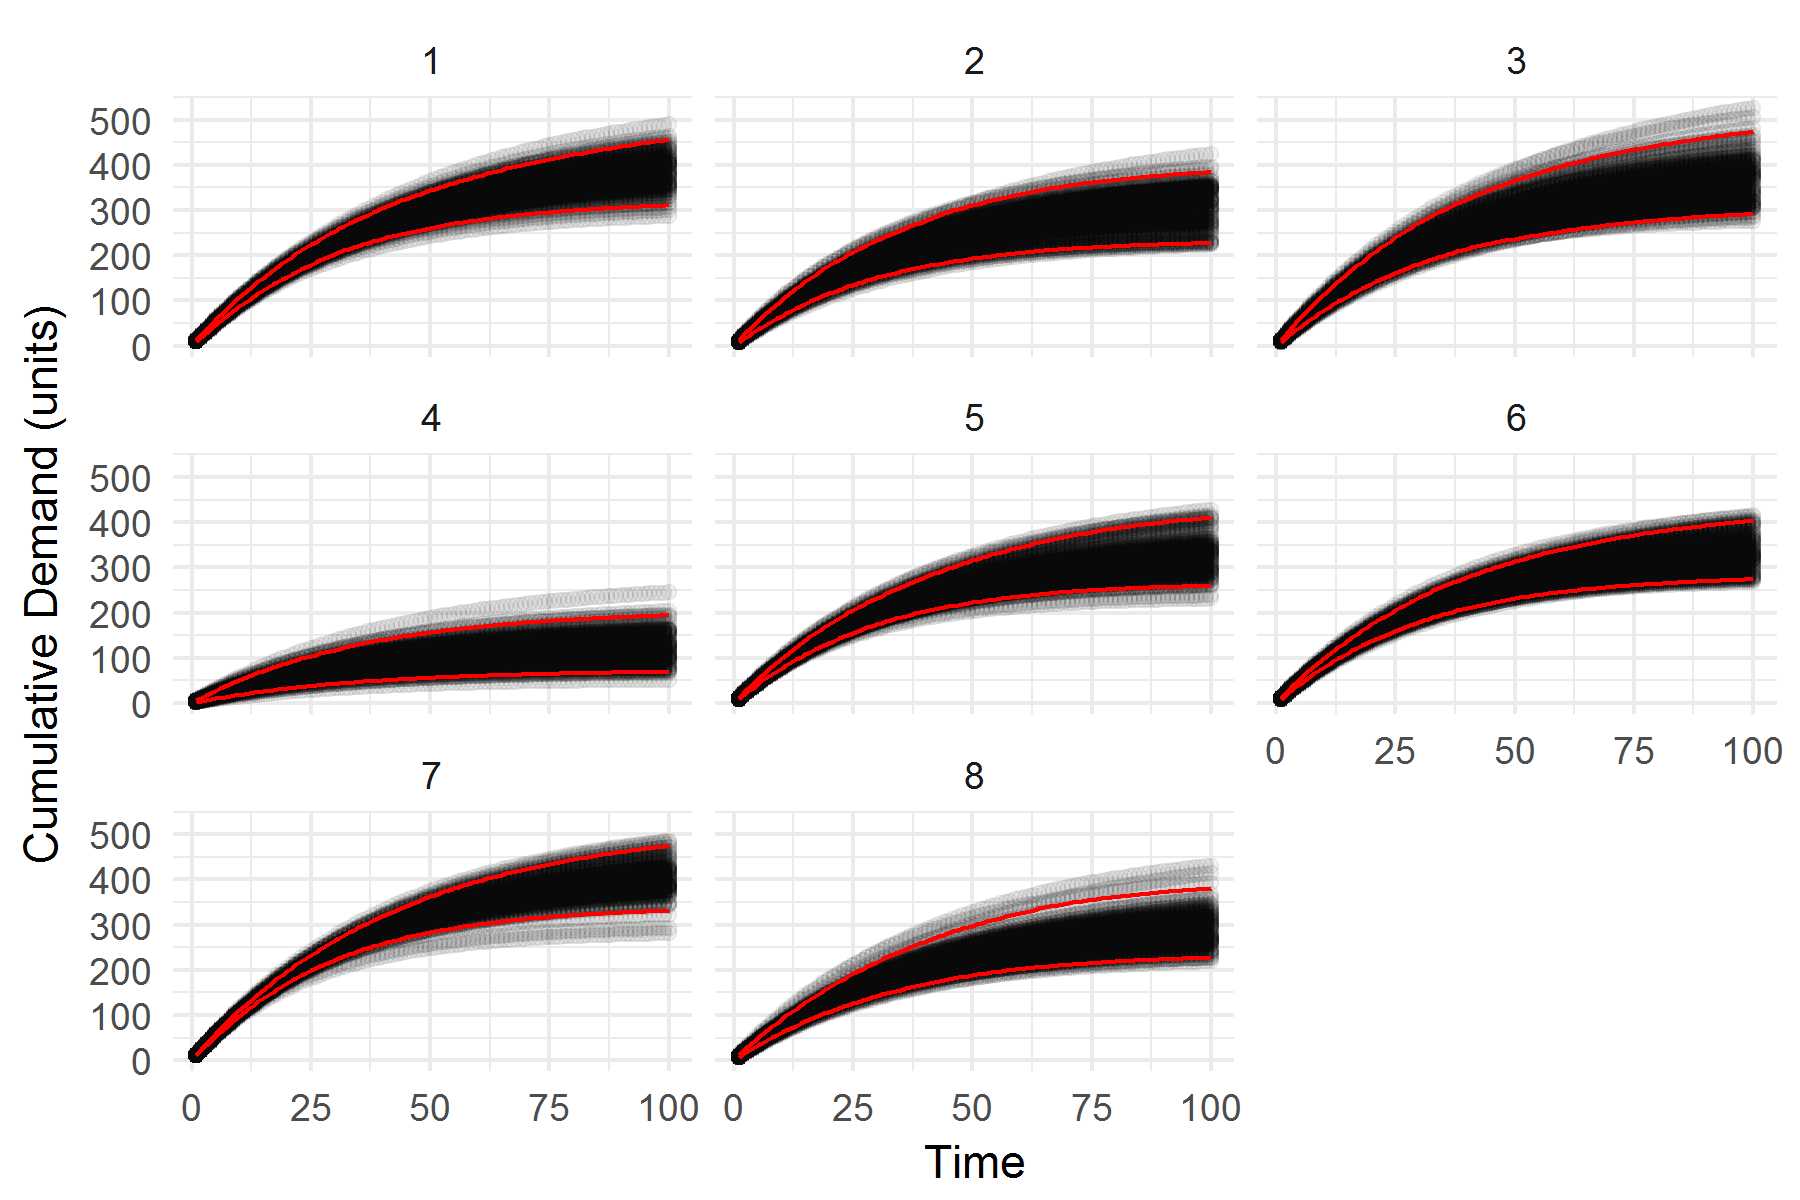
\includegraphics{demand-curve-95pct}
\caption{95\% credible intervals for cumulative demand curve in each region.}  \label{fi:demcurve}
\end{figure}

We determined an appropriate buy by deriving the posterior distribution of the cumulative demand across all regions at time $t = 100$.  The $90^{th}$ percentile of the posterior predictive distribution of demand was \SI{2828} units.  That number was selected as the buy, so $b = 2828$.

The most complicated part of the simulated example was the specification of the rules for fulfillment or orders and transfer between fulfillment centers.  For fulfillment orders, the general strategy is to minimize $\sum_{k = 1}^K \sum_{i = 1}^{n_{kt}} c_1 (f_{tki}, h_{tki})$, the total cost of fulfillment, on any day $t$.  At time points for which all fulfillment centers had sufficient remaining inventory to deliver to all of the ordering households for which it was the closest center, the fulfillment rule was simple --- households receive their order from the closest fulfillment center.  At time points for which fulfillment cannot be satisfied by the fulfillment center closest to a household placing an order, a sequential deterministic rule was used to reassign fulfillment to other centers.  Across all of the fulfillment centers with insufficient inventory to fulfill an order, we calculated the distance from the fulfillment centers with excess inventory to each of the ordering households.  The household with the minimum distance from a fulfillment center with excess inventory was moved from its currently assigned under-stocked fulfillment center to that alternate fulfillment center.

For transfer, inventories were assessed after orders were fulfilled at each time point.  For each fulfillment center, we first calculated its forecasted remaining orders (ignoring the fact that forecasts can be updated dynamically based on observed sales).  Since forecasts are available only at the region level, each fulfillment center was associated with the regions with centroids closest to that fulfillment center.  Referring to Figure~\ref{fi:hhfclocs}, the assignments were as follows: fulfillment center 1 is associated with region 4, fulfillment center 2 is associated with regions 5 and 7, fulfillment center 3 is associated with regions 1 and 8, and fulfillment center 4 is associated with regions 2, 3, and 6.  After calculating forecasted remaining orders, we calculated the difference between that forecast and the number of units remaining in inventory.  If one center was at least 25 units short and another center had at least 25 units too many, a transfer was made.  Transfers were always made from the fulfillment center that was the most over-stocked to the center that was the most under-stocked.  The number of units transferred was the minimum of the number required to meet the forecast needs of the under-stocked fulfillment center or the number of excess units in the over-stocked center.

Finally, we specified the cost functions associated with fulfillment, transfer, and markdowns as follows:

$$c_1 (f, h) = 5 + 5 d(f, h),$$

$$c_2 (u, f_1, f_2) = 4 + 1 u + 5 d(f_1, f_2),$$

\noindent and

$$m (b, d^*) = 29.99 \exp \{- 0.00069 (b - d^*) \}.$$

\noindent where $d(\cdot, \cdot)$ is Euclidean distance.  The value of \SI{29.99} was selected arbitrarily as an AUR without a markdown.  The value of $\delta = 0.00069$ was selected so that an overstock of \SI{1000} units is associated with a markdown of approximately $50\%$ from AUR.

One evaluation of $\mathbb{E}[\nu \mid \alpha_{10}, \alpha_{20}, \ldots, \alpha_{J0}]$ takes approximately 45 seconds on a single AWS processor.  The operation is easily parallelized, but for this proof-of-concept implementation we chose to reduce the set of initial inventory allocations explored and execute the process sequentially.  The set of initial allocations consisted of the $G = 125$ combinations of $\alpha_{10} = 100, 200, \dots, 500$; $\alpha_{20} = 300, 400, \dots, 700$; and $\alpha_{30} = 500, 800, \ldots 900$.  Each combination was assessed using $L = 100$ Monte Carlo simulations.

\subsection{Results}

Because the analysis was performed on a coarse grid, a statistical model was fitted to the observed estimates of expected value to obtain a final estimate of the optimal initial allocation.  Figure~\ref{fi:modelbroad} shows the estimated values of $\mathbb{E}[\nu]$ (points) and fitted model (lines) for selected levels of initial allocation to fulfillment center 1 (rows), fulfillment center 2 (columns), and fulfillment center 3 (x-axis).  In this figure, the y-axis shows the deviation from the optimal estimated point in dollars.  In this figure, the optimal allocation is obtained in the panel with $\alpha_{10} = 400$ (row) and $\alpha_{20} = 600$ (column), and the optimal fitted value is at $\alpha_{30} = 680$.  Using the fitted model to refine the estimate, the optimal point is identified as $\alpha_{10} = 418$, $\alpha_{20} = 571$, $\alpha_{30} = 682$, and $\alpha_{40} = 1157$.

\begin{figure}
\centering
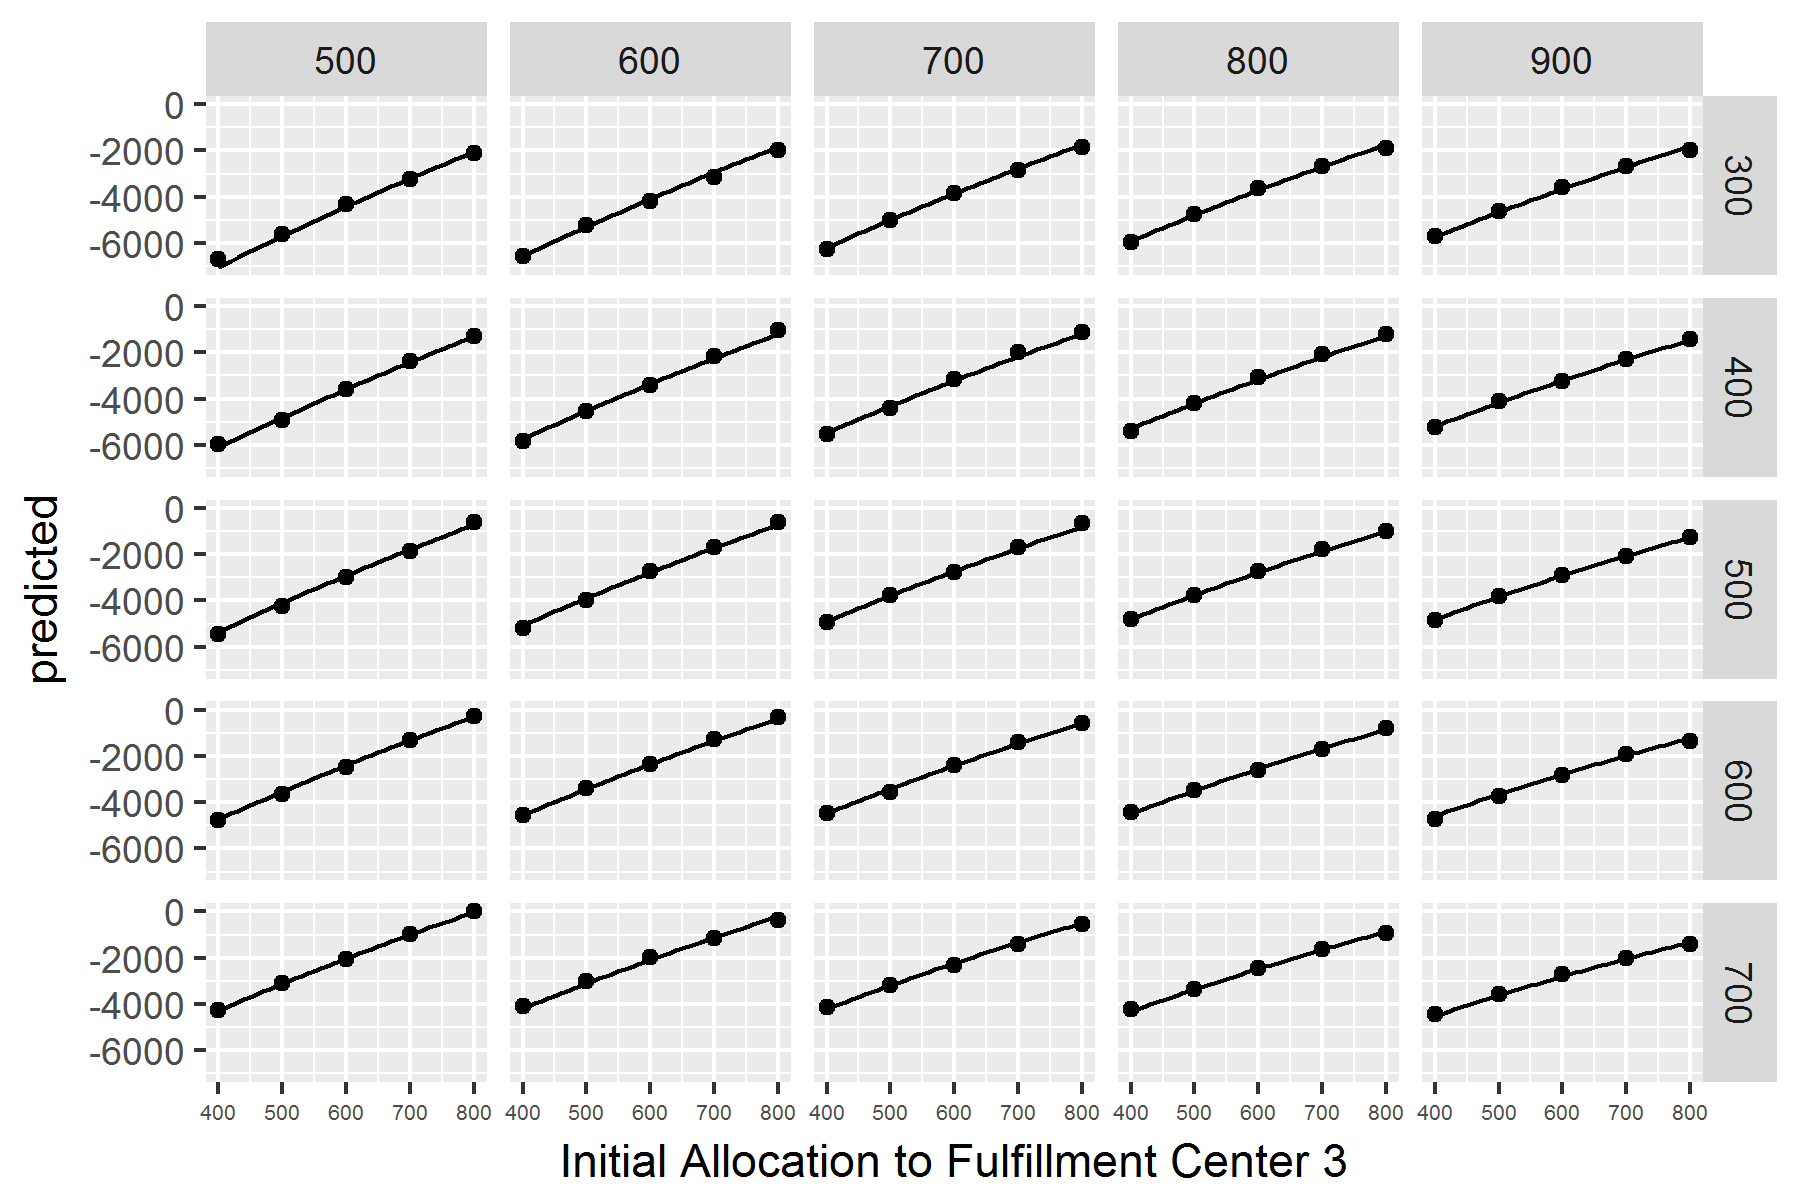
\includegraphics{model-fit-broad}
\caption{Estimated deviation from optimal value (points) and fitted model (lines) for selected levels of allocations to fulfillment centers.}  \label{fi:modelbroad}
\end{figure}


\end{document}  


